% template by Natalia Chernov for the University of Oldenburg

\documentclass[xcolor=table,9pt,aspectratio=169]{beamer}

\usepackage[utf8]{inputenc}

\usepackage{amsmath}
\usepackage{anyfontsize}
\usepackage[english,ngerman]{babel}
\usepackage[autostyle]{csquotes}
\usepackage{datetime}
\usepackage{enumitem}
   \def\labelitemi{--}
   \def\labelitemii{--}
   \def\labelitemiii{--}
\usepackage{helvet}
   \renewcommand{\familydefault}{\sfdefault}
\usepackage{hyperref}
   \urlstyle{same}
\usepackage{lipsum}
\usepackage{listings}
\usepackage{lmodern}
\usepackage{multicol}
\usepackage{multirow}
\usepackage{smartdiagram}
\usepackage{tikz}
\usepackage{xcolor}

\definecolor{uolblue}{RGB}{0,62,107}

\definecolor{blue1}{RGB}{0,78,159}
\definecolor{blue2}{RGB}{0,171,217}
\definecolor{blue3}{RGB}{91,197,242}
\definecolor{blue4}{RGB}{161,217,248}

\definecolor{green1}{RGB}{0,120,120}
\definecolor{green2}{RGB}{0,168,121}
\definecolor{green3}{RGB}{148,193,28}
\definecolor{green4}{RGB}{199,211,0}

\definecolor{orange1}{RGB}{213,59,10}
\definecolor{orange2}{RGB}{238,113,0}
\definecolor{orange3}{RGB}{243,145,0}
\definecolor{orange4}{RGB}{253,195,0}

\definecolor{gr}{RGB}{191,191,191}
\definecolor{grcode}{RGB}{190,190,190}

\lstdefinestyle{mystyle}{
   backgroundcolor=\color{grcode},
   commentstyle=\color{blue1},
   numberstyle=\tiny\color{blue1},
   basicstyle=\ttfamily\footnotesize,
   breakatwhitespace=false,
   breaklines=true,
   captionpos=b,
   keepspaces=true,
   numbers=left,
   numbersep=5pt,
   showspaces=false,
   showstringspaces=false,
   showtabs=false,
   tabsize=2
}

\setbeameroption{hide notes}
% \setbeameroption{show only notes}
% \setbeameroption{show notes on second screen=right}

\setbeamertemplate{frametitle}{\color{uolblue}\fontsize{12}{20}\selectfont{\insertframetitle}}

\pgfdeclareimage[width=0.145\paperwidth]{logo}{figures/logo_uol_negative}
\pgfdeclareimage[width=0.072\paperwidth]{logo_small}{figures/logo_uol_negative}

\defbeamertemplate*{background canvas}{default_page}
{%
\begin{tikzpicture}
   \useasboundingbox (0,0) rectangle (\the\paperwidth,\the\paperheight);
   \filldraw[fill=uolblue,fill opacity=1,draw=none] (0,0) rectangle (0.119\paperwidth,\the\paperheight);
   \filldraw[fill=blue2,fill opacity=1,draw=none] (0.119\paperwidth,0) -- (0.119\paperwidth,0.565\paperheight) arc (117.2:180:0.6\paperwidth) -- cycle;
   \pgftext[at=\pgfpoint{10}{\the\paperheight-11.5},left,top]{\pgfsetfillopacity{1}\pgfuseimage{logo_small}};
\end{tikzpicture}
}
\defbeamertemplate*{background canvas}{titlepage_image}
{
\begin{tikzpicture}
   \useasboundingbox (0,0) rectangle (\the\paperwidth,\the\paperheight);
   \filldraw[fill=uolblue,fill opacity=1,draw=none] (0,0) rectangle (\the\paperwidth,\the\paperheight);
   \filldraw[fill=blue2,fill opacity=1,draw=none] (\the\paperwidth,0) -- (\the\paperwidth,0.66\paperheight) arc (90:180:0.6\paperwidth) -- cycle;
   \pgftext[at=\pgfpoint{14}{\the\paperheight-17.5},left,top]{\pgfsetfillopacity{1}\pgfuseimage{logo}};
\end{tikzpicture}
}
\BeforeBeginEnvironment{frame}{%
   \setbeamertemplate{background canvas}[default_page]%
}
\makeatletter
\define@key{beamerframe}{titlepage_image}[true]{%
   \setbeamercovered{invisible}%
   \setbeamertemplate{background canvas}[titlepage_image]%
}
\makeatother%

\setbeamertemplate{footline}
{
   \leavevmode
   \hbox{
   \hspace*{.025\paperwidth}\begin{beamercolorbox}[wd=.094\paperwidth,ht=2.25ex,dp=1ex,left]{}
   ~

   \vspace*{.042\paperheight}
      \fontsize{4.4}{5.9}\selectfont\color{white}\textbf{Folie \insertframenumber}\newline\insertdate
   \vspace*{.026\paperheight}
   \end{beamercolorbox}
   \hspace*{.05\paperwidth}\begin{beamercolorbox}
   [wd=.79\paperwidth,ht=2.25ex,dp=1ex,left]{}
   ~

   \vspace*{.042\paperheight}
      \fontsize{4.4}{5.9}\selectfont\color{black}\textbf{Einführung in die Logik -- Ex-Post-Evaluation}\newline\color{gray}\insertauthor~--~Fakultät IV, Institut für Philosophie
   \vspace*{.026\paperheight}
   \end{beamercolorbox}
   }
   \vskip0pt
}

\setbeamerfont{title}{size={\fontsize{22}{25}}}
\setbeamerfont{subtitle}{size={\fontsize{12}{14}}}
\setbeamerfont{author}{size={\fontsize{9}{11}}}
\setbeamerfont{date}{size={\fontsize{9}{11}}}
\setbeamercolor{title}{fg=white}
\setbeamercolor{subtitle}{fg=white}
\setbeamercolor{author}{fg=white}
\setbeamercolor{date}{fg=white}
\setbeamercolor{color_Logo-Platzhalter}{fg=white,bg=gray!40}

\defbeamertemplate*{title page}{customized}[1][]
{  \vspace*{20mm}
   \hspace*{-22.5mm}
   \begin{minipage}{\textwidth}
   \usebeamerfont{title}\usebeamercolor[fg]{title}\inserttitle\par
   \bigskip
   \usebeamerfont{subtitle}\usebeamercolor[fg]{subtitle}\insertsubtitle\par
   \bigskip
   \usebeamerfont{author}\usebeamercolor[fg]{author}\insertauthor\par
   \bigskip
   \usebeamerfont{date}\usebeamercolor[fg]{date}\insertdate\par
   \end{minipage}
}
\setbeamertemplate{navigation symbols}{}
\setbeamersize{text margin left=0.17\paperwidth,text margin right=0.04\paperwidth}

\title{Einführung in die Logik}
\subtitle{Befragung zur Klausurvorbereitung}
\author{Alexander Max Bauer und Mark Siebel}
\date{WiSe 2024/2025}
% \date{\renewcommand{\dateseparator}{.}\ddmmyyyydate\today}

\begin{document}
{
\setbeamertemplate{footline}{}
\begin{frame}[titlepage_image]
   \maketitle
\end{frame}
}


%%%%%%%%%%%%%%%%%%%%%%%%
% FOLIE 2 – GLIEDERUNG %
%%%%%%%%%%%%%%%%%%%%%%%%
\begin{frame}{\vspace*{10mm}Gliederung}
\begin{itemize}
   \item[1] Material
   \item[2] Teilnehmer:innen
   \begin{itemize}
      \item Alter und Geschlecht
      \item Vorkenntnisse
   \end{itemize}
   \item[3] Klausurergebnisse
   \begin{itemize}
      \item Module
      \item Noten
   \end{itemize}
   \item[4] Lehrveranstaltungen
   \begin{itemize}
      \item Vorlesung
      \item Tutorium
      \item Zusatztutorium
   \end{itemize}
\end{itemize}
\end{frame}


%%%%%%%%%%%
% FOLIE 3 %
%%%%%%%%%%%
\begin{frame}{\vspace*{10mm}Gliederung}
\begin{itemize}
   \item[5] Klausurvorbereitung
   \begin{itemize}
      \item Selbsteinschätzung
      \item Vorbereitungszeit
      \item Vorbereitungsmittel
      \item Übungszettel
      \item Einzel- und Gruppenarbeit
   \end{itemize}
   \item[6] Klausursituation
   \begin{itemize}
      \item Zeit
      \item Konzentration
      \item Schwierigkeit
   \end{itemize}
\end{itemize}
\end{frame}


%%%%%%%%%%%%%%%%%%%%%%
% FOLIE 4 – MATERIAL %
%%%%%%%%%%%%%%%%%%%%%%
\begin{frame}{\vspace*{10mm}1\hspace*{1em}Material}
LimeSurvey-Umfrage-Struktur, Daten, Do-File für die Analyse mit Stata und Folien\\sind verfügbar unter:

\bigskip
\url{https://github.com/alephmembeth/survey-logic-2025}
\end{frame}


%%%%%%%%%%%%%%%%%%%%%%%%%%%%%%
% FOLIE 5 – TEILNEHMER:INNEN %
%%%%%%%%%%%%%%%%%%%%%%%%%%%%%%
\begin{frame}{\vspace*{10mm}2\hspace*{1em}Teilnehmer:innen}
\textbf{Alter}\\

\smallskip
$\text{Mean} \approx 22,590$

\bigskip
\textbf{Geschlecht}\\

\medskip
\begin{tabular}{lcc}
   \arrayrulecolor{blue2}\hline
                & Absolute     & Relative     \\
                & Häufigkeit   & Häufigkeit   \\
   \hline\hline
   Weiblich     &  62          &  52,99       \\
   Nichtbinär   &   2          &   1,71       \\
   Männlich     &  53          &  45,30       \\
   \hline
                & 117          & 100,00       \\
   \hline
\end{tabular}
\end{frame}


%%%%%%%%%%%
% FOLIE 6 %
%%%%%%%%%%%
\begin{frame}{\vspace*{10mm}2\hspace*{1em}Teilnehmer:innen}
\textbf{Vorkenntnisse}\\

\medskip
\begin{tabular}{lcc}
   \arrayrulecolor{blue2}\hline
          & Absolute     & Relative     \\
          & Häufigkeit   & Häufigkeit   \\
   \hline\hline
   Nein   &  88          &  73,95       \\
   Ja     &  31          &  26,05       \\
   \hline
          & 120          & 100,00       \\
   \hline
\end{tabular}
\end{frame}


%%%%%%%%%%%%%%%%%%%%%%%%%%%%%%%
% FOLIE 7 – KLAUSURERGEBNISSE %
%%%%%%%%%%%%%%%%%%%%%%%%%%%%%%%
\begin{frame}{\vspace*{10mm}3\hspace*{1em}Klausurergebnisse}
\textbf{Module}\\

\medskip
\begin{tabular}{lcc}
   \arrayrulecolor{blue2}\hline
            & Absolute     & Relative     \\
            & Häufigkeit   & Häufigkeit   \\
   \hline\hline
   phi130   &  76          &  63,33       \\
   pb036    &  44          &  36,67       \\
   \hline
            & 121          & 100,00       \\
   \hline
\end{tabular}
\end{frame}


%%%%%%%%%%%
% FOLIE 8 %
%%%%%%%%%%%
\begin{frame}{\vspace*{10mm}3\hspace*{1em}Klausurergebnisse}
\textbf{Noten}\\
\begin{multicols}{2}
   \begin{center}
      \frame{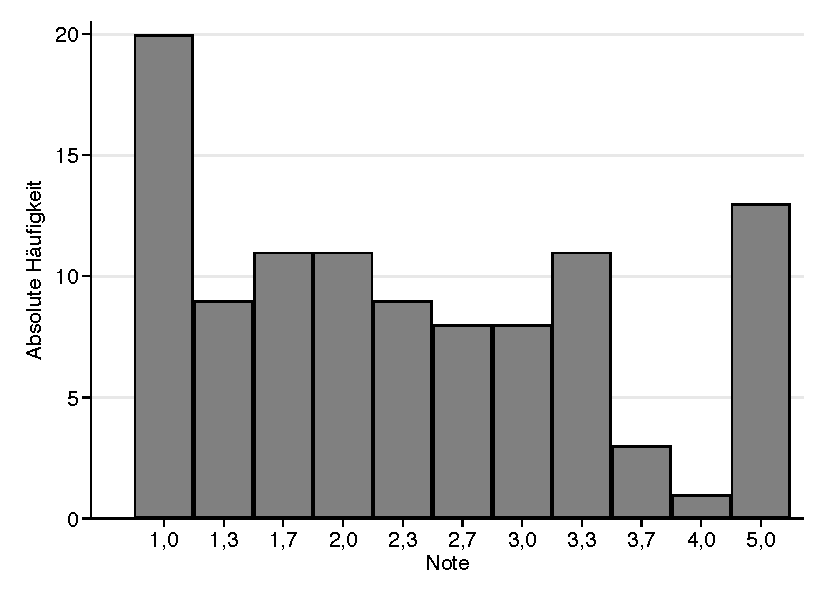
\includegraphics[width=0.75\linewidth]{figures/figure_note_1.pdf}}\\Erste Klausur\\
      \frame{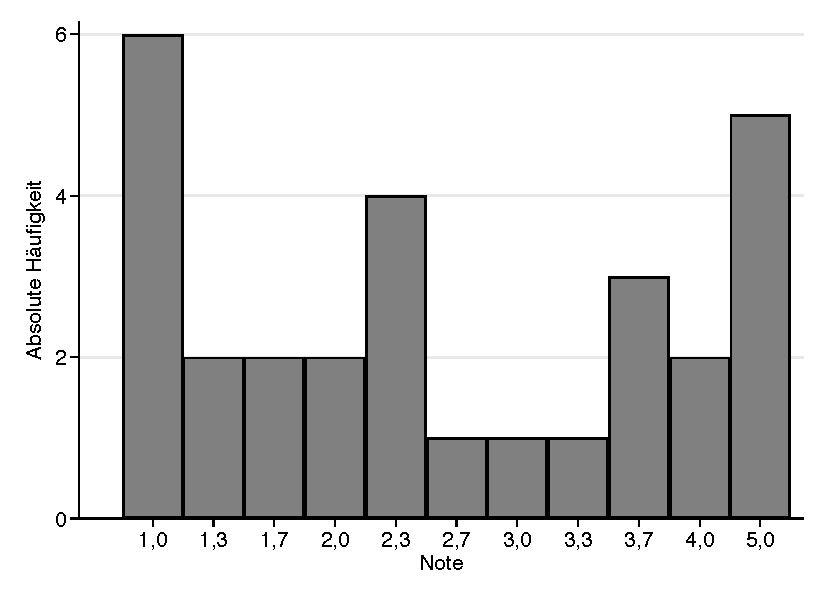
\includegraphics[width=0.75\linewidth]{figures/figure_note_2.pdf}}\\Zweite Klausur\\
   \end{center}
\end{multicols}
\end{frame}


%%%%%%%%%%%%%%%%%%%%%%%%%%%%%%%%%
% FOLIE 9 – LEHRVERANSTALTUNGEN %
%%%%%%%%%%%%%%%%%%%%%%%%%%%%%%%%%
\begin{frame}{\vspace*{10mm}4\hspace*{1em}Lehrveranstaltungen}
\textbf{Vorlesung}\\
\begin{multicols}{2}
   \begin{center}
      \frame{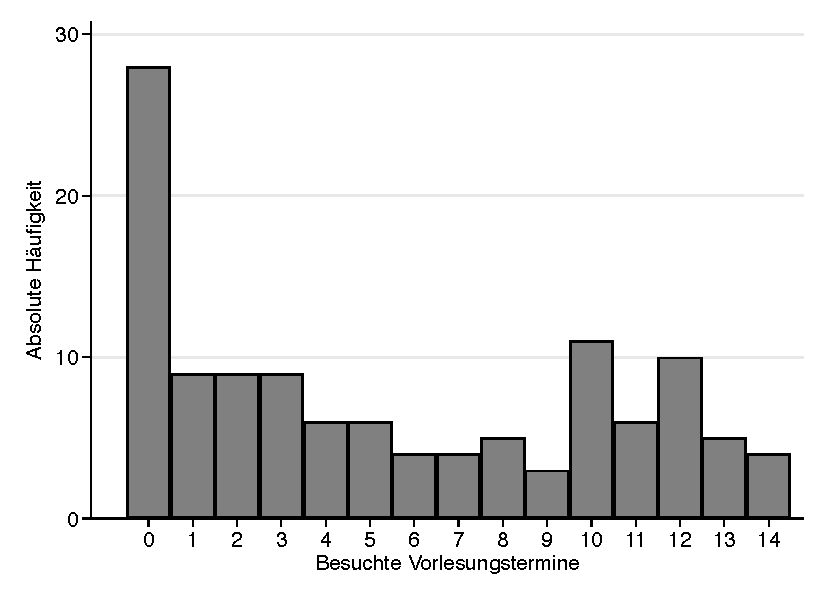
\includegraphics[width=0.75\linewidth]{figures/figure_vorlesungpraesenz.pdf}}\\
      \frame{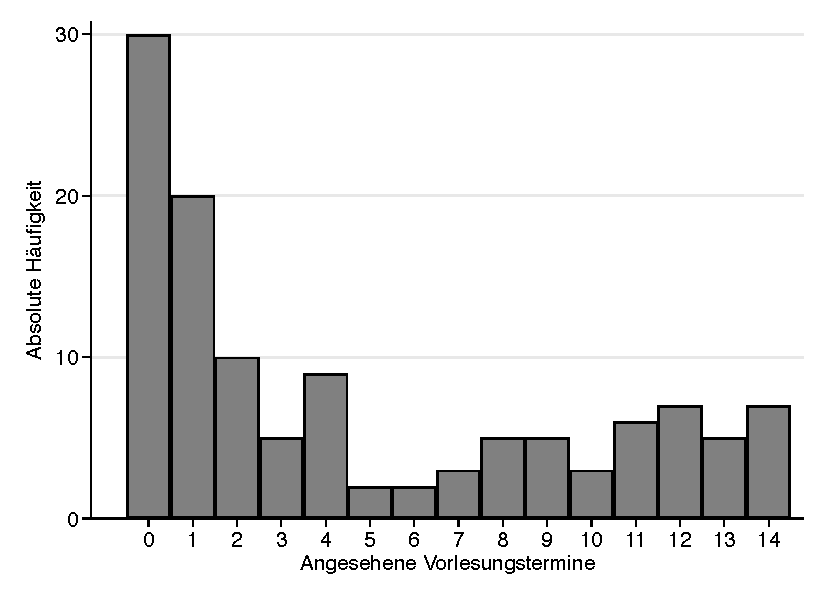
\includegraphics[width=0.75\linewidth]{figures/figure_vorlesungvideo.pdf}}\\
   \end{center}
\end{multicols}
\textbf{Frage:} Wie viele Termine der Vorlesung haben Sie in Präsenz besucht [als Aufzeichnung angesehen]?
\end{frame}


%%%%%%%%%%%%
% FOLIE 10 %
%%%%%%%%%%%%
\begin{frame}{\vspace*{10mm}4\hspace*{1em}Lehrveranstaltungen}
\textbf{Tutorium}\\

\smallskip
\begin{center}
   \frame{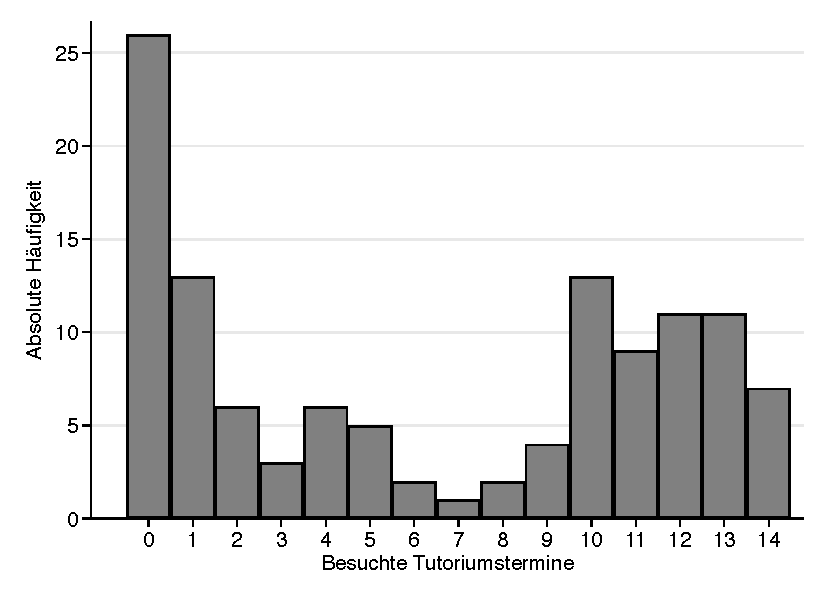
\includegraphics[width=0.4\linewidth]{figures/figure_tutorium.pdf}}\\
\end{center}

\bigskip
\textbf{Frage:} Wie viele Termine des Tutoriums haben Sie besucht?
\end{frame}


%%%%%%%%%%%%
% FOLIE 11 %
%%%%%%%%%%%%
\begin{frame}{\vspace*{10mm}4\hspace*{1em}Lehrveranstaltungen}
\textbf{Zusatztutorium}\\

\medskip
\begin{tabular}{lcc}
   \arrayrulecolor{blue2}\hline
          & Absolute     & Relative     \\
          & Häufigkeit   & Häufigkeit   \\
   \hline\hline
   Nein   &  95          &  79,83       \\
   Ja     &  24          &  20,17       \\
   \hline
          & 119          & 100,00       \\
   \hline
\end{tabular}

\bigskip
\textbf{Frage:} Haben Sie an einem Zusatztutorium teilgenommen?
\end{frame}


%%%%%%%%%%%%
% FOLIE 12 %
%%%%%%%%%%%%
\begin{frame}{\vspace*{10mm}5\hspace*{1em}Klausurvorbereitung}
\textbf{Selbsteinschätzung}\\

\smallskip
\begin{center}
   \frame{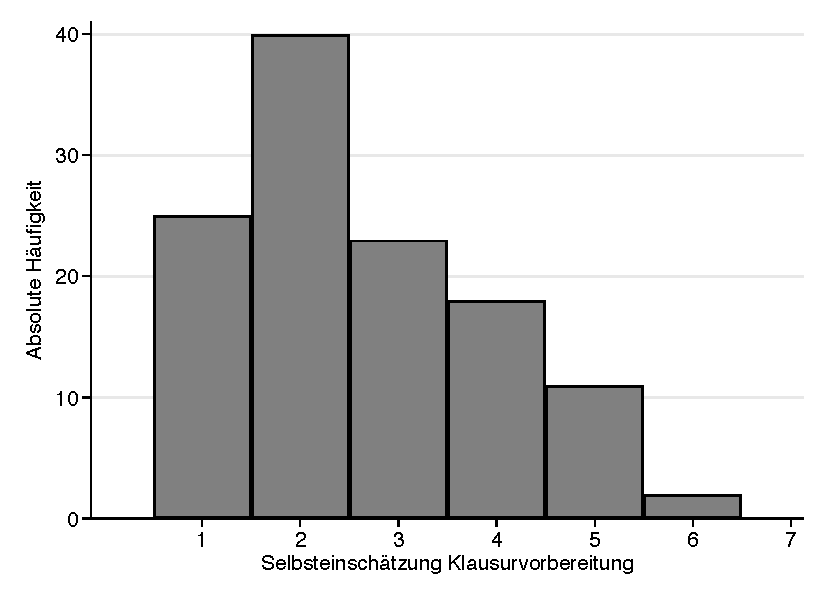
\includegraphics[width=0.4\linewidth]{figures/figure_einschaetzung.pdf}}\\
\end{center}

\bigskip
\textbf{Frage:} Wie gut haben Sie sich Ihrer Meinung nach auf die Klausur vorbereitet? Beantworten Sie diese Frage bitte auf einer Skala von 1 (sehr gut) bis 7 (gar nicht gut).
\end{frame}


%%%%%%%%%%%%
% FOLIE 13 %
%%%%%%%%%%%%
\begin{frame}{\vspace*{10mm}5\hspace*{1em}Klausurvorbereitung}
\textbf{Vorbereitungszeit}\\

\smallskip
\begin{center}
   \frame{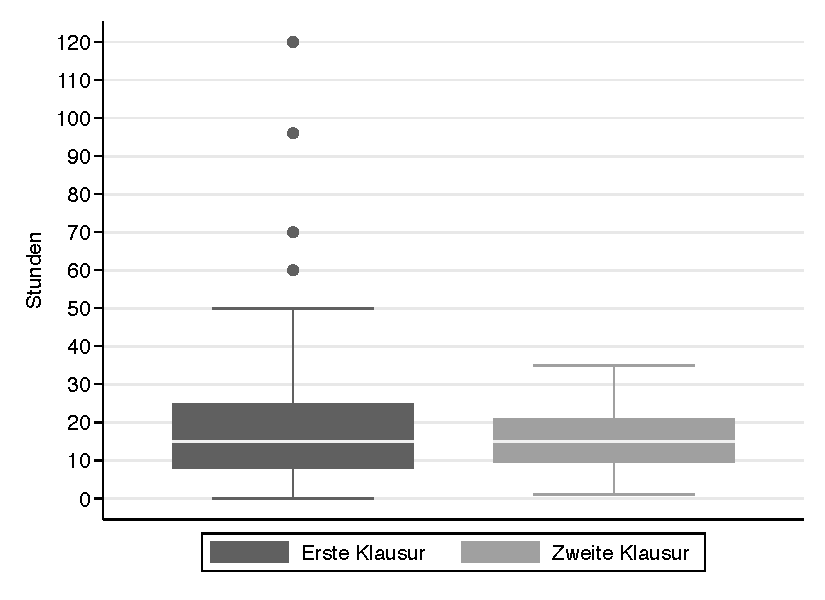
\includegraphics[width=0.4\linewidth]{figures/figure_zeit.pdf}}\\
\end{center}
\textbf{Klausur 1:} $\text{Mean} \approx 21,363, \text{Median} = 15$; \textbf{Klausur 2:} $\text{Mean} \approx 15,429, \text{Median} = 15$

\bigskip
\textbf{Frage:} Wie viele Stunden haben Sie vor der ersten [zweiten] Klausur insgesamt für die Klausurvorbereitung genutzt?
\end{frame}


%%%%%%%%%%%%
% FOLIE 14 %
%%%%%%%%%%%%
\begin{frame}{\vspace*{10mm}5\hspace*{1em}Klausurvorbereitung}
\textbf{Vorbereitungsmittel}\\

\medskip
\begin{tabular}{lcc}
   \arrayrulecolor{blue2}\hline
                                       & Absolute     & Relative     \\
                                       & Häufigkeit   & Häufigkeit   \\
   \hline\hline
   Keine Vorbereitung                  &   1          &   0,85       \\
   Übungsklausuren ansehen             &   1          &   0,85       \\
   Übungsklausuren bearbeiten          &  19          &  16,24       \\
   Übungsaufgaben ansehen              &   8          &   6,84       \\
   Übungsaufgaben bearbeiten           &  70          &  59,83       \\
   Zusätzliches Lernmaterial ansehen   &  18          &  15,38       \\
   \hline
                                       & 117          & 100,00       \\
   \hline
\end{tabular}

\bigskip
\textbf{Frage:} Wie haben Sie sich auf die Klausur vorbereitet? Mehrere Antworten sind möglich.
\end{frame}


%%%%%%%%%%%%
% FOLIE 15 %
%%%%%%%%%%%%
\begin{frame}{\vspace*{10mm}5\hspace*{1em}Klausurvorbereitung}
\textbf{Übungszettel}\\
\begin{multicols}{2}
   \begin{center}
      \frame{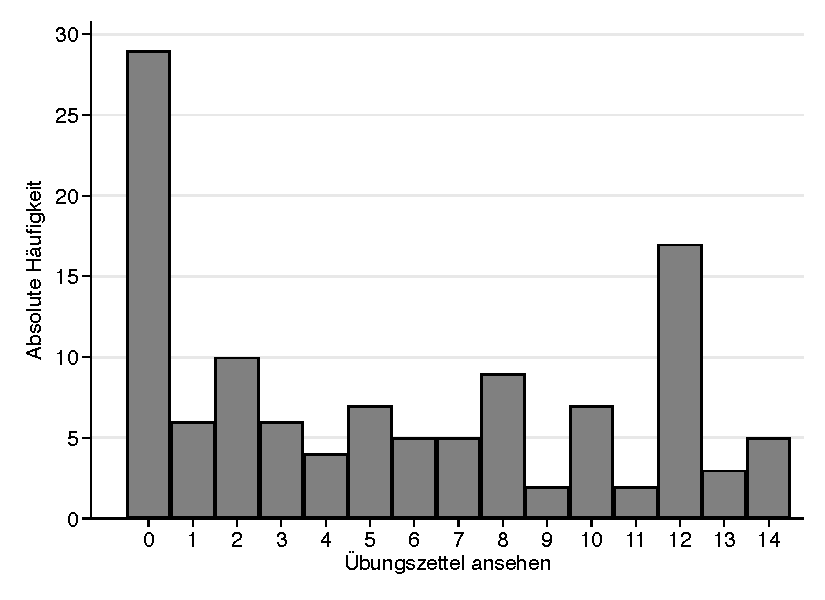
\includegraphics[width=0.75\linewidth]{figures/figure_uebungansehen.pdf}}\\
      \frame{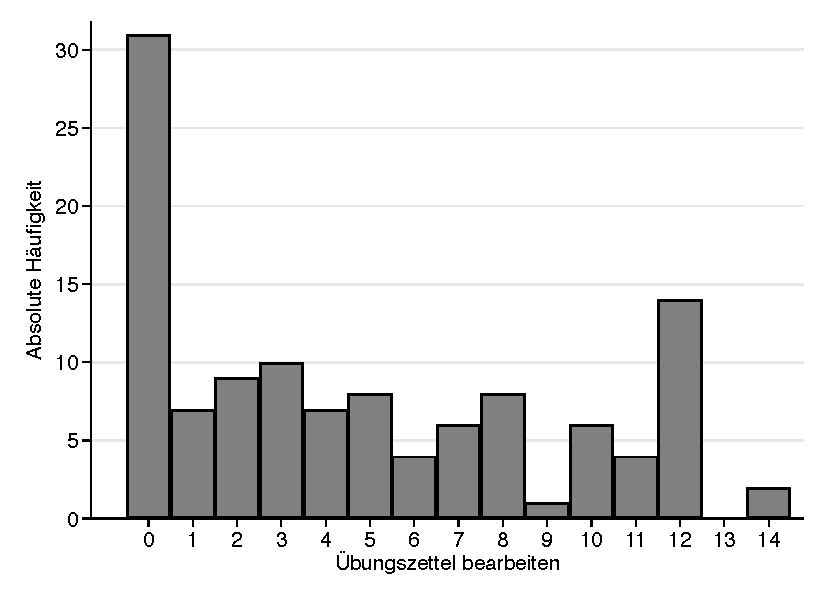
\includegraphics[width=0.75\linewidth]{figures/figure_uebungbearbeiten.pdf}}\\
   \end{center}
\end{multicols}
\textbf{Frage:} Wie viele der Übungszettel haben Sie versucht [sich] in der Vorlesungszeit (also nicht erst zur direkten Klausurvorbereitung) zu lösen [angesehen]?
\end{frame}


%%%%%%%%%%%%
% FOLIE 16 %
%%%%%%%%%%%%
\begin{frame}{\vspace*{10mm}5\hspace*{1em}Klausurvorbereitung}
\textbf{Einzel- und Gruppenarbeit}\\

\medskip
\begin{tabular}{lcc}
   \arrayrulecolor{blue2}\hline
                                      & Absolute     & Relative     \\
                                      & Häufigkeit   & Häufigkeit   \\
   \hline\hline
   Ganz oder überwiegend alleine      &  89          &  76,07       \\
   Manchmal zusammen mit anderen      &  19          &  16,24       \\
   Überwiegend zusammen mit anderen   &   9          &   7,69       \\
   \hline
                                      & 117          & 100,00       \\
   \hline
\end{tabular}

\bigskip
\textbf{Frage:} Haben Sie sich auf die Klausur eher alleine oder zusammen mit anderen vorbereitet?
\end{frame}


%%%%%%%%%%%%%%%%%%%%%%%%%%%%%%%
% FOLIE 17 – KLAUSURSITUATION %
%%%%%%%%%%%%%%%%%%%%%%%%%%%%%%%
\begin{frame}{\vspace*{10mm}6\hspace*{1em}Klausursituation}
\textbf{Zeit}\\
\begin{multicols}{2}
   \begin{center}
      \frame{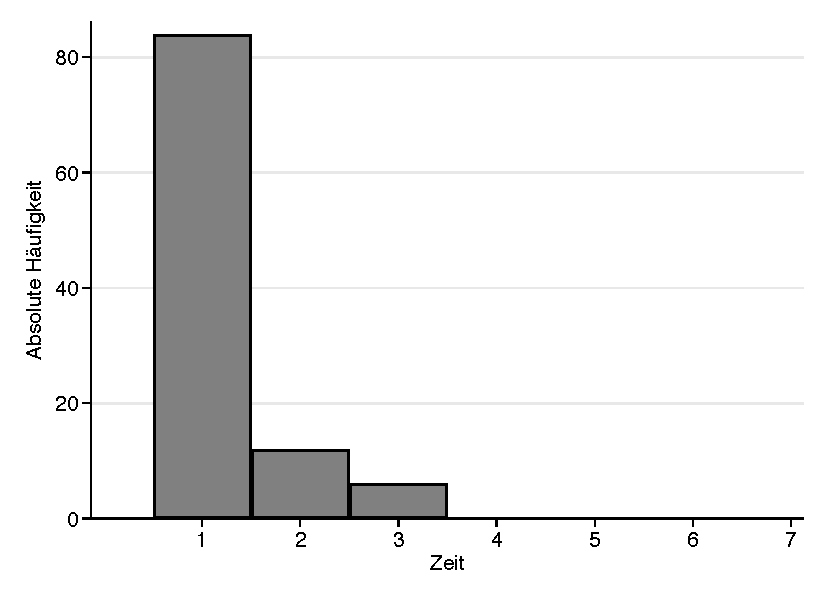
\includegraphics[width=0.75\linewidth]{figures/figure_zeit_1.pdf}}\\Erste Klausur\\
      \frame{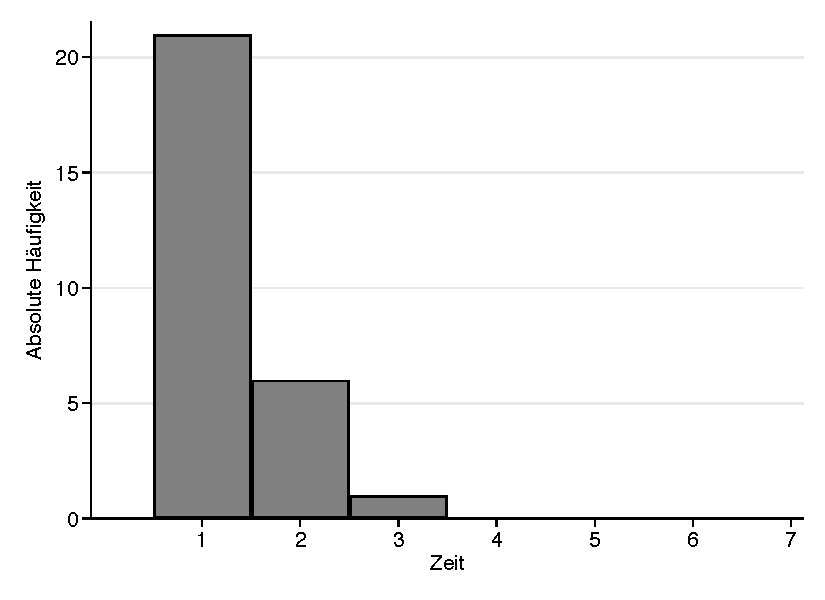
\includegraphics[width=0.75\linewidth]{figures/figure_zeit_2.pdf}}\\Zweite Klausur\\
   \end{center}
\end{multicols}
\textbf{Frage:} Wie gut kamen Sie mit der Dauer der ersten [zweiten] Klausur zurecht?
\end{frame}


%%%%%%%%%%%%
% FOLIE 18 %
%%%%%%%%%%%%
\begin{frame}{\vspace*{10mm}6\hspace*{1em}Klausursituation}
\textbf{Konzentration}\\
\begin{multicols}{2}
   \begin{center}
      \frame{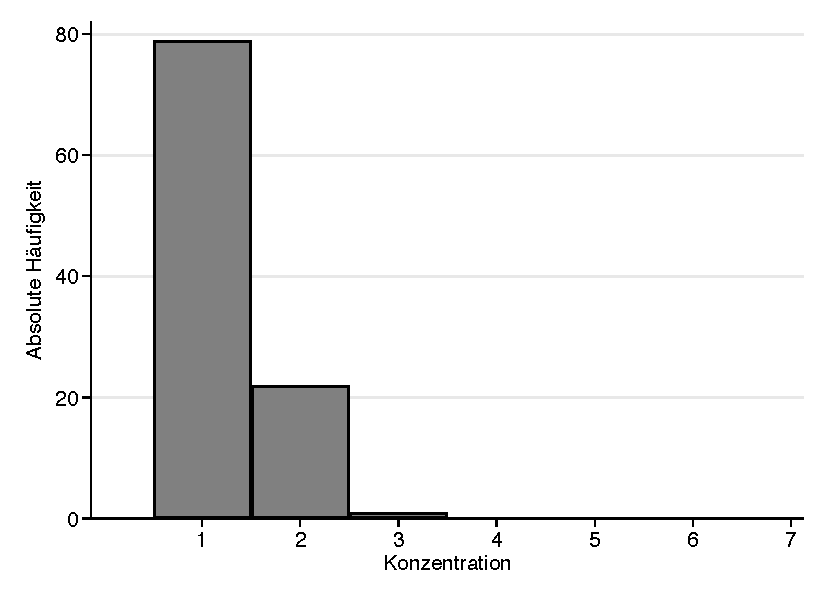
\includegraphics[width=0.75\linewidth]{figures/figure_konzentration_1.pdf}}\\Erste Klausur\\
      \frame{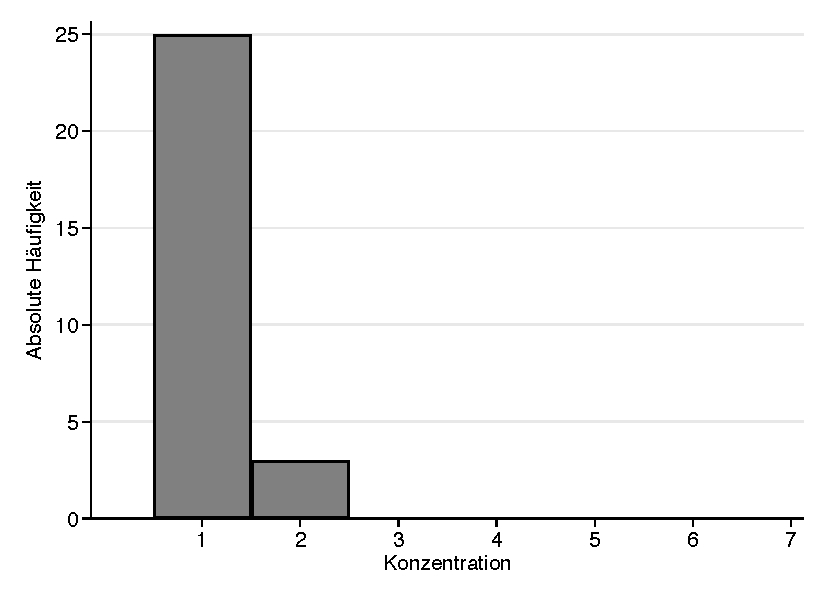
\includegraphics[width=0.75\linewidth]{figures/figure_konzentration_2.pdf}}\\Zweite Klausur\\
   \end{center}
\end{multicols}
\textbf{Frage:} Wie gut konnten Sie sich während der ersten [zweiten] Klausur konzentrieren?
\end{frame}


%%%%%%%%%%%%
% FOLIE 19 %
%%%%%%%%%%%%
\begin{frame}{\vspace*{10mm}6\hspace*{1em}Klausursituation}
\textbf{Konzentration}\\
\begin{multicols}{2}
   \begin{center}
      \frame{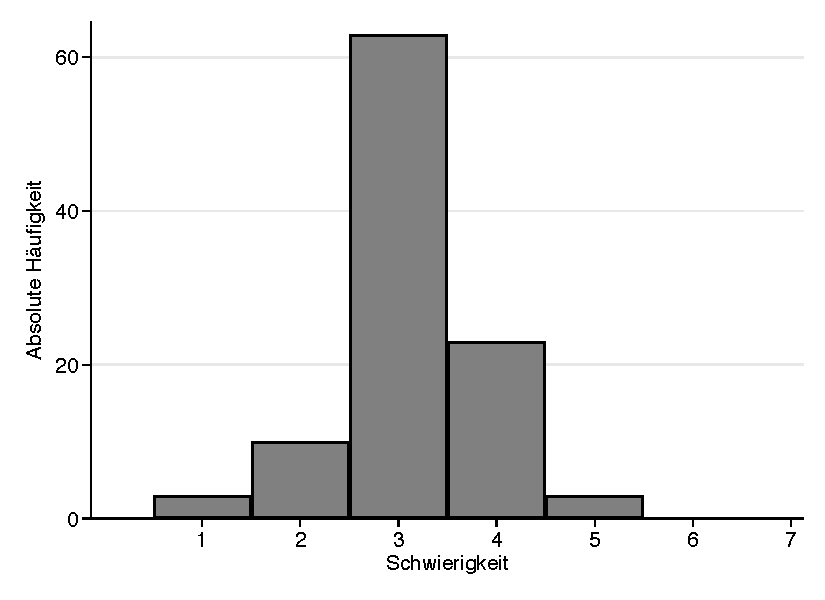
\includegraphics[width=0.75\linewidth]{figures/figure_schwierigkeit_1.pdf}}\\Erste Klausur\\
      \frame{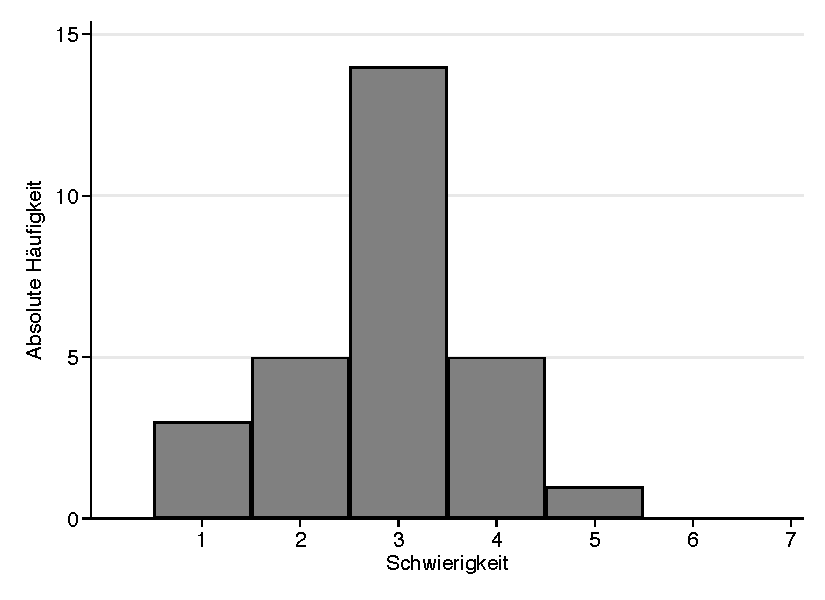
\includegraphics[width=0.75\linewidth]{figures/figure_schwierigkeit_2.pdf}}\\Zweite Klausur\\
   \end{center}
\end{multicols}
\textbf{Frage:} Wie schwierig erschien Ihnen die erste [zweite] Klausur?
\end{frame}


\end{document}
